\documentclass{article}

\usepackage{geometry}
\usepackage{gbt7714}
\usepackage{xeCJK}
\usepackage{booktabs}       % professional-quality tables
\usepackage{amsfonts}       % blackboard math symbols
\usepackage{subfig}
\usepackage{amsmath}
\usepackage{graphicx}
\usepackage{float}
\usepackage{svg}

\graphicspath{{assets/}}


\linespread{1.5}
\geometry{a4paper, left=2.5cm, right=2.5cm, top=2.5cm, bottom=2.5cm}
\bibliographystyle{gbt7714-numerical}   
\title{基于潜在正则化对抗的特高压直流换流阀声音异常检测}

\begin{document}
\maketitle

\begin{abstract}

The converter valve is a core component of high-voltage direct current (HVDC) transmission systems, responsible for converting direct current (AC) to alternating current (DC) and ensuring efficient and stable long-distance transmission and distribution of electric power. However, the occurrence of faults in actual systems is infrequent, making the comprehensive collection of anomaly samples highly challenging. Supervised detection methods rely on a large amount of labeled normal and abnormal data for training, while traditional anomaly detection methods based on reconstruction or adversarial learning struggle to separate normal and abnormal data in the latent space, failing to achieve efficient detection.
To address these issues, this paper proposes a new unsupervised anomaly detection method called Latent Regularization Adversarial Anomaly Detection (LRAAD). The training approach of LRAAD is similar to that of generative adversarial networks (GANs), but LRAAD uses an encoder to serve as a discriminator. The discriminator in a GAN maps the input spectrogram to a scalar value representing the probability that the input image is real data. In the LRAAD model, the discriminator task of the encoder is more complex, it maps the input spectrogram to a latent space and determines the authenticity of the input spectrogram through the Kullback-Leibler (KL) divergence between the latent representation and a standard normal distribution. This method allows the encoder to learn the key features of the input spectrogram and map them to the latent space, enabling the generator to produce samples that better match the real data distribution.
Experiments were conducted on a dataset of real-world sound recordings from converter stations to validate the proposed method. The results show that the LRAAD method significantly outperforms other baseline models in terms of AUC and p-AUC metrics for anomaly detection tasks, demonstrating its effectiveness and practicality. This provides a new solution for anomaly sound detection in the field of converter valve condition monitoring.

\end{abstract}


关键字：异常声音检测, 无监督学习, 对抗学习, 潜在变量正则化对抗

\section{Introduction}
With the continuous development and upgrading of power systems, ultra-high voltage (UHV) transmission technology has been widely applied globally. As an essential component of the power system, the operational state of UHV converter stations is directly related to the reliability and stability of power transmission. However, key equipment such as converter valves may experience anomalies like partial discharge during operation, leading to system performance degradation or even severe faults. To ensure the safe operation of the power system, accurate and efficient anomaly detection methods are particularly important. Traditional anomaly detection methods for converter valves mainly rely on monitoring physical parameters such as vibration and temperature, while methods based on sound signals have gradually gained attention \cite{AR-AD}.

In anomaly detection, obtaining anomaly data is often difficult because faults in actual systems occur infrequently and in diverse forms, making the collection of comprehensive anomaly samples highly challenging. Supervised detection methods rely on a large amount of labeled normal and abnormal data for training, but due to the scarcity of anomaly data, these methods show limitations in practical applications and struggle to handle previously unseen anomalies.

Traditional anomaly detection methods mainly rely on manual inspection and simple statistical analysis, which are inadequate for handling complex and variable operating conditions and fail to meet the real-time requirements of practical applications. In recent years, anomaly detection methods based on machine learning and deep learning have gradually emerged, showing high detection accuracy and good adaptability. However, existing anomaly detection methods based on reconstruction or adversarial learning struggle to effectively separate normal and abnormal data in the latent space, limiting their practical application effectiveness.

To address the aforementioned issues, this paper proposes a new unsupervised anomaly detection method called Latent Regularization Adversarial Anomaly Detection (LRAAD). This method conducts adversarial learning in the latent space domain, using an encoder to act as a discriminator. It minimizes the Kullback-Leibler (KL) divergence between the latent representation of normal data and the standard normal distribution, assigning high scores, while maximizing the KL divergence for generated data, assigning low scores. This enables the encoder to effectively distinguish between normal and abnormal data.

The LRAAD model consists of two main modules: an encoder and a generator. The encoder receives the input spectrogram and converts it into a representation in the latent space, optimizing the latent space distribution by minimizing the KL divergence between the latent representation of normal data and the standard normal distribution. The generator maps the latent variables back to the spectrogram domain, generating the most realistic spectrograms possible and continually improving its generation capability through adversarial learning. The joint training of the encoder and generator enables the model to effectively detect anomalies under different load conditions.

The dataset used in the experiments comes from actual sound data of converter valves at a ±800kV UHV converter station in China. Based on the apparent power of the converter valve during operation, the dataset is divided into six subsets corresponding to apparent power ranges from 400 MVA to 1000 MVA. These data include sounds from normal operation as well as fault features such as partial discharge, providing rich samples for model training and validation.

The main contributions of this paper include the following: 
\begin{enumerate} 
\item A new anomaly detection method, LRAAD, is proposed, achieving effective separation of normal and abnormal data through adversarial learning in the latent space domain. 
\item The model is validated using actual sound data from a UHV converter station, and experimental results show that the LRAAD method exhibits high anomaly detection accuracy and robustness under different load conditions. 
\end{enumerate}

The structure of this paper is arranged as follows: Chapter 2 introduces related research work and background knowledge; Chapter 3 discusses the mechanism of sound generation in converter valves and analyzes fault sounds; Chapter 4 describes the design and implementation of the LRAAD model in detail, including the architecture and training methods of the encoder and generator; Chapter 5 presents the experimental setup and dataset division, and analyzes and discusses the experimental results; Chapter 6 summarizes the research work and proposes future research directions.

\section{Related Work}

Since 2020, DCASE Task 2\cite{DCASE2020Task2,DCASE2021Task2,DCASE2022Task2,DCASE2023Task2} has aimed to develop a self-supervised machine anomaly sound detection model based on deep learning\cite{DeepLearning-1,DeepLearning-2,DeepLearning-3} to achieve real-time monitoring and fault warning of industrial equipment. Recently, many self-supervised anomaly sound detection methods based on deep learning have been developed, including methods based on autoencoders\cite{AE-AD,AE-AD-2,CAE-AD,VAE-AD,VAE-AD-2,SAE-AD}, flow-based anomaly detection methods\cite{NF-AD,DifferNet,CFlow-AD}, anomaly detection methods based on generative adversarial networks\cite{AnoGAN,EGBAD,f-AnoGAN,GANomaly,AEGAN-AD}, and anomaly detection methods based on autoregressive networks\cite{AR-AD,WaveNet-AD}.

\subsection{Autoencoder-based Methods}

Autoencoder (AE) is a neural network structure commonly used in unsupervised learning, widely applied in anomaly detection. An autoencoder trains a neural network to compress input data into a low-dimensional latent space and then restores it to its original dimension through a decoder. The goal of the autoencoder is to minimize reconstruction error, meaning the difference between the input data and the reconstructed data should be as small as possible. Autoencoder-based anomaly detection methods utilize this characteristic to identify anomalies by analyzing reconstruction errors.

In the research on anomaly detection methods based on autoencoders, researchers have mainly focused on traditional autoencoders (AE)\cite{AE-AD} and variational autoencoders (VAE)\cite{VAE,VAE-AD}. For example, Sabokrou et al.\cite{AE-AD} proposed an anomaly detection method based on autoencoders, which trains an autoencoder to learn the feature representation of normal data and then uses reconstruction error to identify anomalies. Similarly, Huang et al.\cite{AE-AD-2} proposed a visual anomaly detection (VAD) method based on AE. This method first introduces an automatic encoding transformer (AT) to widen the anomaly score gap between normal and abnormal samples, then uses an AE model to learn the high-level semantic features of normal samples, thus obtaining the latent representation of normal samples. Duman et al.\cite{CAE-AD} proposed an anomaly detection method based on convolutional autoencoders (CAE), which trains a CAE model to learn the feature representation of normal data and then uses reconstruction error to identify anomalies. These methods have achieved some success in anomaly detection tasks, but due to the limitations of autoencoders, they perform poorly in learning complex data distributions, resulting in high reconstruction errors and difficulty in accurate model fitting.

Anomaly detection methods based on variational autoencoders (VAE)\cite{VAE-AD,VAE-AD-2} improve model generalization by introducing latent variables and KL divergence to learn the latent representation of data. For example, An et al.\cite{VAE-AD} proposed an anomaly detection method based on VAE, which trains a VAE model to learn the latent representation of normal data and then uses KL divergence to measure the difference between normal and abnormal data.


Methods based on autoencoders perform well in detecting stable sound signals; however, due to the diversity of equipment operating conditions, actual sound signals exhibit significant variations. These methods perform poorly in learning good feature probability distributions, resulting in high reconstruction errors and difficulty in accurate model fitting\cite{DeepLearning-4}.

\subsection{GAN-based Methods}

Generative Adversarial Networks (GANs)\cite{GAN}, introduced by Ian Goodfellow et al. in 2014, are a powerful generative model that uses two competing neural networks (a generator and a discriminator) trained adversarially to achieve data generation and feature learning. GAN-based anomaly detection methods leverage the generative capability of GANs and the discriminative power of the discriminator. The generator creates data, and the discriminator identifies anomalies, making this approach one of the significant methods in the field of anomaly detection in recent years\cite{GAN-BASED-AD-REVIEW}.

GAN-based anomaly detection methods utilize the generative capability of GANs to identify anomalies by analyzing the differences between generated data and actual data. Schlegl et al. proposed the AnoGAN\cite{AnoGAN} method, which learns the distribution of normal data using a GAN generator and detects anomalies through the differences between generated and actual data. However, this method requires learning the mapping from images to the latent space during inference, which is time-consuming. To address this issue, Schlegl et al.\cite{f-AnoGAN} improved AnoGAN by proposing the f-AnoGAN method, which significantly increases detection speed by learning the mapping from images to the latent space. Akcay et al.\cite{GANomaly} proposed a new encoder-decoder-encoder architecture model called GANomaly, which uses reconstruction loss, latent representation loss, and adversarial loss to train the model and compute anomaly scores. Experiments show that it outperforms state-of-the-art GAN-based and traditional autoencoder-based anomaly detection methods. Jiang et al.\cite{AEGAN-AD} proposed an unsupervised model called AEGAN-AD for machine audio anomaly detection using GANs. The study shows that by introducing a discriminator to provide feature-level guidance, the AEGAN-AD model can understand representations more deeply, addressing the issue of the encoder potentially reconstructing abnormal signals.

\subsection{Flow-based Methods}

Flow-based models are a type of generative model that have emerged in recent years. They map complex data distributions to simple distributions (typically Gaussian) through invertible transformations, which have a computable Jacobian determinant, enabling precise calculation of data probability density. Flow-based models excel in anomaly detection because they can directly estimate the probability density of input data, and subsequently determine whether the data is anomalous based on the probability density values.

In recent years, anomaly detection methods based on flow models have been extensively researched. For example, Rudolph et al.\cite{DifferNet} proposed a semi-supervised defect detection method called DifferNet, which uses multi-scale feature extractors to handle the high dimensionality of images, allowing normalized flows to assign meaningful likelihoods. Gudovskiy et al.\cite{CFlow-AD} proposed a real-time unsupervised anomaly detection model CFLOW-AD, which uses conditional normalized flows for anomaly localization. Rudolph et al.\cite{CSFlow} introduced a novel fully convolutional cross-scale normalized flow (CS-Flow) for image-based defect detection. This method efficiently detects image anomalies by jointly processing multi-scale feature maps to model the distribution of defect-free image data.

The advantages of flow models lie in their high-precision probability estimation capabilities, enabling accurate modeling of data distributions in high-dimensional spaces. Additionally, the invertibility of flow models ensures lossless data transformations, making them perform well in generation and reconstruction tasks. In anomaly detection, flow models can accurately distinguish between normal and abnormal data, improving detection accuracy and reliability. However, flow models also face challenges and limitations. First, the training process typically requires significant computational resources and time, especially for high-dimensional data. Second, flow models demand careful model structure and parameter settings, often requiring extensive experimentation to adjust hyperparameters. Furthermore, flow models may be less effective with discrete and sparse data compared to continuous and dense data.


\subsection{AutoRegressive-based Methods}

An autoregressive model (AR) is a statistical model that uses the historical values of a sequence to predict its current or future values. Widely used in time series analysis, autoregressive models forecast by modeling the dependencies within the data sequence. Anomaly detection methods based on autoregressive models leverage this sequential dependency to identify anomalies within the data, making them particularly suitable for anomaly detection in time series data.

Anomaly detection methods based on autoregressive models mainly focus on the WaveNet model\cite{WaveNet-AD,AR-AD}. Rushe et al.\cite{AR-AD} proposed applying the WaveNet architecture to audio anomaly detection and experimentally compared its performance with benchmark autoencoder models, showing that WaveNet outperforms in almost all cases. This study is significant as it extends the application field of the WaveNet architecture and demonstrates its effectiveness in audio anomaly detection. Hayashi et al.\cite{WaveNet-AD} proposed a WaveNet-based method for detecting anomalous sound events. This method uses WaveNet as a convolutional neural network-based generative model to model various acoustic patterns in public spaces. When the model detects unknown acoustic patterns, it identifies them as anomalous sound events.



\section{Converter Valve Sound Analysis}

特高压换流阀作为电力系统中至关重要的设备，其运行状态直接影响整个系统的可靠性和稳定性。在运行过程中，换流阀会产生多种声音，这些声音不仅反映了设备的正常工作状态，也可能揭示潜在的故障隐患。理解换流阀声音的产生机理及故障声音特征，对于异常检测和故障诊断具有重要意义。

\subsection{换流阀声音产生机理}

换流阀在其运行过程中会产生多种声音，这些声音主要来源于以下几个方面：

\textbf{电磁噪声}是换流阀运行中最常见的声音之一。换流阀内的大量电力电子元件（如晶闸管、IGBT等）在高频开关过程中会产生电磁噪声。这些噪声由电磁波在周围介质中的传播和元件间的电磁相互作用引起，频率较高且音量不大。电磁噪声通常表现为高频的“嗡嗡”声，持续且均匀。

\textbf{机械振动}也是换流阀声音的重要来源。换流阀的开关动作会导致其内部结构部件的机械振动，尤其是在电流突变时，电动力作用会使换流阀的结构件（如冷却系统、支撑架等）发生微小的机械位移，从而发出振动噪声。这类噪声通常频率较低，但振幅较大，表现为低频的“嗡嗡”声或“咚咚”声。

\textbf{冷却系统噪声}也是换流阀运行中不可忽视的部分。为了确保在高负荷运行时的温度控制，换流阀通常配备复杂的冷却系统（如风冷、液冷等）。冷却系统中的风机、泵等设备在运行时会产生明显的噪声，这部分噪声相对稳定，但随着换流阀负载的变化，其音量和频率也会有所不同，通常表现为稳定的“隆隆”声或“呼呼”声。

\textbf{局部放电噪声}是换流阀在高压环境下可能发生的一种特殊声音。局部放电是一种电气故障现象，通常伴随有高频的放电噪声。局部放电噪声由电离过程中的电流脉冲产生，频率范围较广且具有随机性，通常表现为不连续的高频“噼啪”声。

\subsection{ 换流阀故障声音分析}

不同故障状态下，换流阀会产生特定的声音特征，识别这些声音特征对于异常检测和故障诊断具有重要意义。以下是几种常见故障及其对应的声音特征：

\textbf{局部放电故障}是高压换流阀常见的故障类型之一。局部放电会产生高频的尖锐噪声，类似于“噼啪”声。这种声音通常是不连续的，频率较高（几千赫兹到几十千赫兹），具有明显的随机性和瞬时性。局部放电故障的主要原因包括绝缘材料老化、受潮、局部破损等，这些因素导致局部电场增强，使介质局部电离并产生放电现象。

\textbf{机械故障}会导致换流阀内机械部件的异常振动，发出低频的振动噪声，类似于“嗡嗡”声。这种声音往往是持续的，且音量可能随负载变化而变化。机械故障的原因可能包括固定部件松动、机械磨损、冷却系统故障等，这些问题会导致机械部件振动异常，从而产生明显的低频噪声。

\textbf{冷却系统故障}也会引起特定的声音变化。冷却系统故障会导致风机或泵的运行异常，产生持续的、较大的噪声，类似于“隆隆”声。冷却系统故障的原因可能包括冷却液流动受阻、风机叶片损坏、泵运行不正常等，这些问题会导致冷却系统运行异常，从而产生显著的噪声变化。

\textbf{电磁干扰故障}可能导致高频噪声的增加，表现为持续的高频“滋滋”声。这种声音的频率较高且较稳定，通常伴随着电气设备的开关动作频繁出现。电磁干扰故障的原因可能包括电力电子元件开关频率异常、接触不良等，这些问题会导致电磁干扰增加，从而产生高频噪声。

\section{提出的方法}

生成对抗网络（GAN）\cite{GAN}由Goodfellow等人于2014年提出，是一种通过对抗训练的方式来学习数据分布的生成模型。生成对抗网络由两个神经网络组成：生成器（Generator）和判别器（Discriminator）。判别器的目标是尽可能准确地判断输入数据是真实数据还是生成数据，而生成器的目标是尽可能生成判别器无法区分来源的数据。这两个目标不同的网络不断地进行交替训练，当最后收敛时，生成器可以生成与真实数据分布相似的数据。

LRAAD的训练方式与生成对抗网络类似，但是LRAAD使用编码器来充当判别器的作用。生成对抗网络的判别器将输入的频谱图映射到一个标量值，表示输入图像是真实数据的概率。而编码器在LRAAD模型中的判别任务是更加复杂的，它将输入的频谱图映射到潜在空间，并通过潜在表示与标准正态分布的KL散度来判别输入频谱图的真实性。这种判别方式使得编码器学习到输入频谱图的关键特征，并将其映射到潜在空间，使得生成器能够生成更加符合真实数据分布的样本。


\subsection{模型架构设计}


\subsubsection{编码器}

LRAAD的编码器充当判别器的作用。不同于生成对抗网络的判别器，生成对抗网络的判别器将输入的频谱图映射到一个标量值，表示输入图像是真实数据的概率。而编码器在LRAAD模型中的判别任务是更加复杂的，它需要将输入的频谱图映射到潜在空间，并通过潜在表示与标准正态分布的KL散度来判别输入频谱图的真实性。这种判别任务需要编码器学习到输入频谱图的关键特征，并将其映射到潜在空间，以便后续的生成器能够生成尽可能真实的频谱图。

\begin{figure}[h]
    \centering
    
\includegraphics[width=0.45\textwidth]{./assets/encoder.pdf}
    \caption{The architecture of the encoder $E$}
    \label{fig:encoder}
\end{figure}

编码器的最后一层输出不同于常规的全连接层，如图\ref{fig:encoder}所示。它采用的是均值和方差参数来表示潜在空间的分布，这是基于变分自编码器（Variational Autoencoder，VAE）的思想。通过这种设计，编码器不仅可以生成潜在表示，还能够学习到潜在空间的分布信息，使得潜在表示可以与标准正态分布进行比较。这种比较主要通过KL散度来衡量，KL散度小表示潜在表示接近标准正态分布，反之则表示潜在表示与标准正态分布的分布差异较大。潜在变量$z$的KL散度的计算公式如下：

\begin{equation}
    D_{KL}(q(z|x)||p(z)) = \frac{1}{2} \sum_{i=1}^{N}(\sigma_i^2 + \mu_i^2 - \log(\sigma_i^2) - 1)
\end{equation}

编码器在训练过程中，通过最小化正常数据的潜在表示与标准正态分布之间的KL散度，来学习将正常数据映射到接近标准正态分布的潜在空间。与此同时，学习将异常数据(生成器生成的数据)的潜在表示映射到偏离标准正态分布的潜在空间区域。这种训练方式使得编码器能够更好地区分正常数据和异常数据，因为正常数据在潜在空间中更加紧密地分布，而异常数据则会显著地偏离标准正态分布。

\subsubsection{生成器}

生成器的结构与解码器类似。生成器的输入是编码器生成的潜在变量$z$，输出是生成的频谱图。生成器的目标是通过学习将潜在变量映射到与正常数据频谱图相似的图像，从而提供优质的正常数据样本来优化编码器的学习过程。生成器的训练与编码器交替进行，利用对抗学习的框架来不断提高生成器的生成能力。

\begin{figure}[H]
    \centering
    \def\svgwidth{\textwidth}
    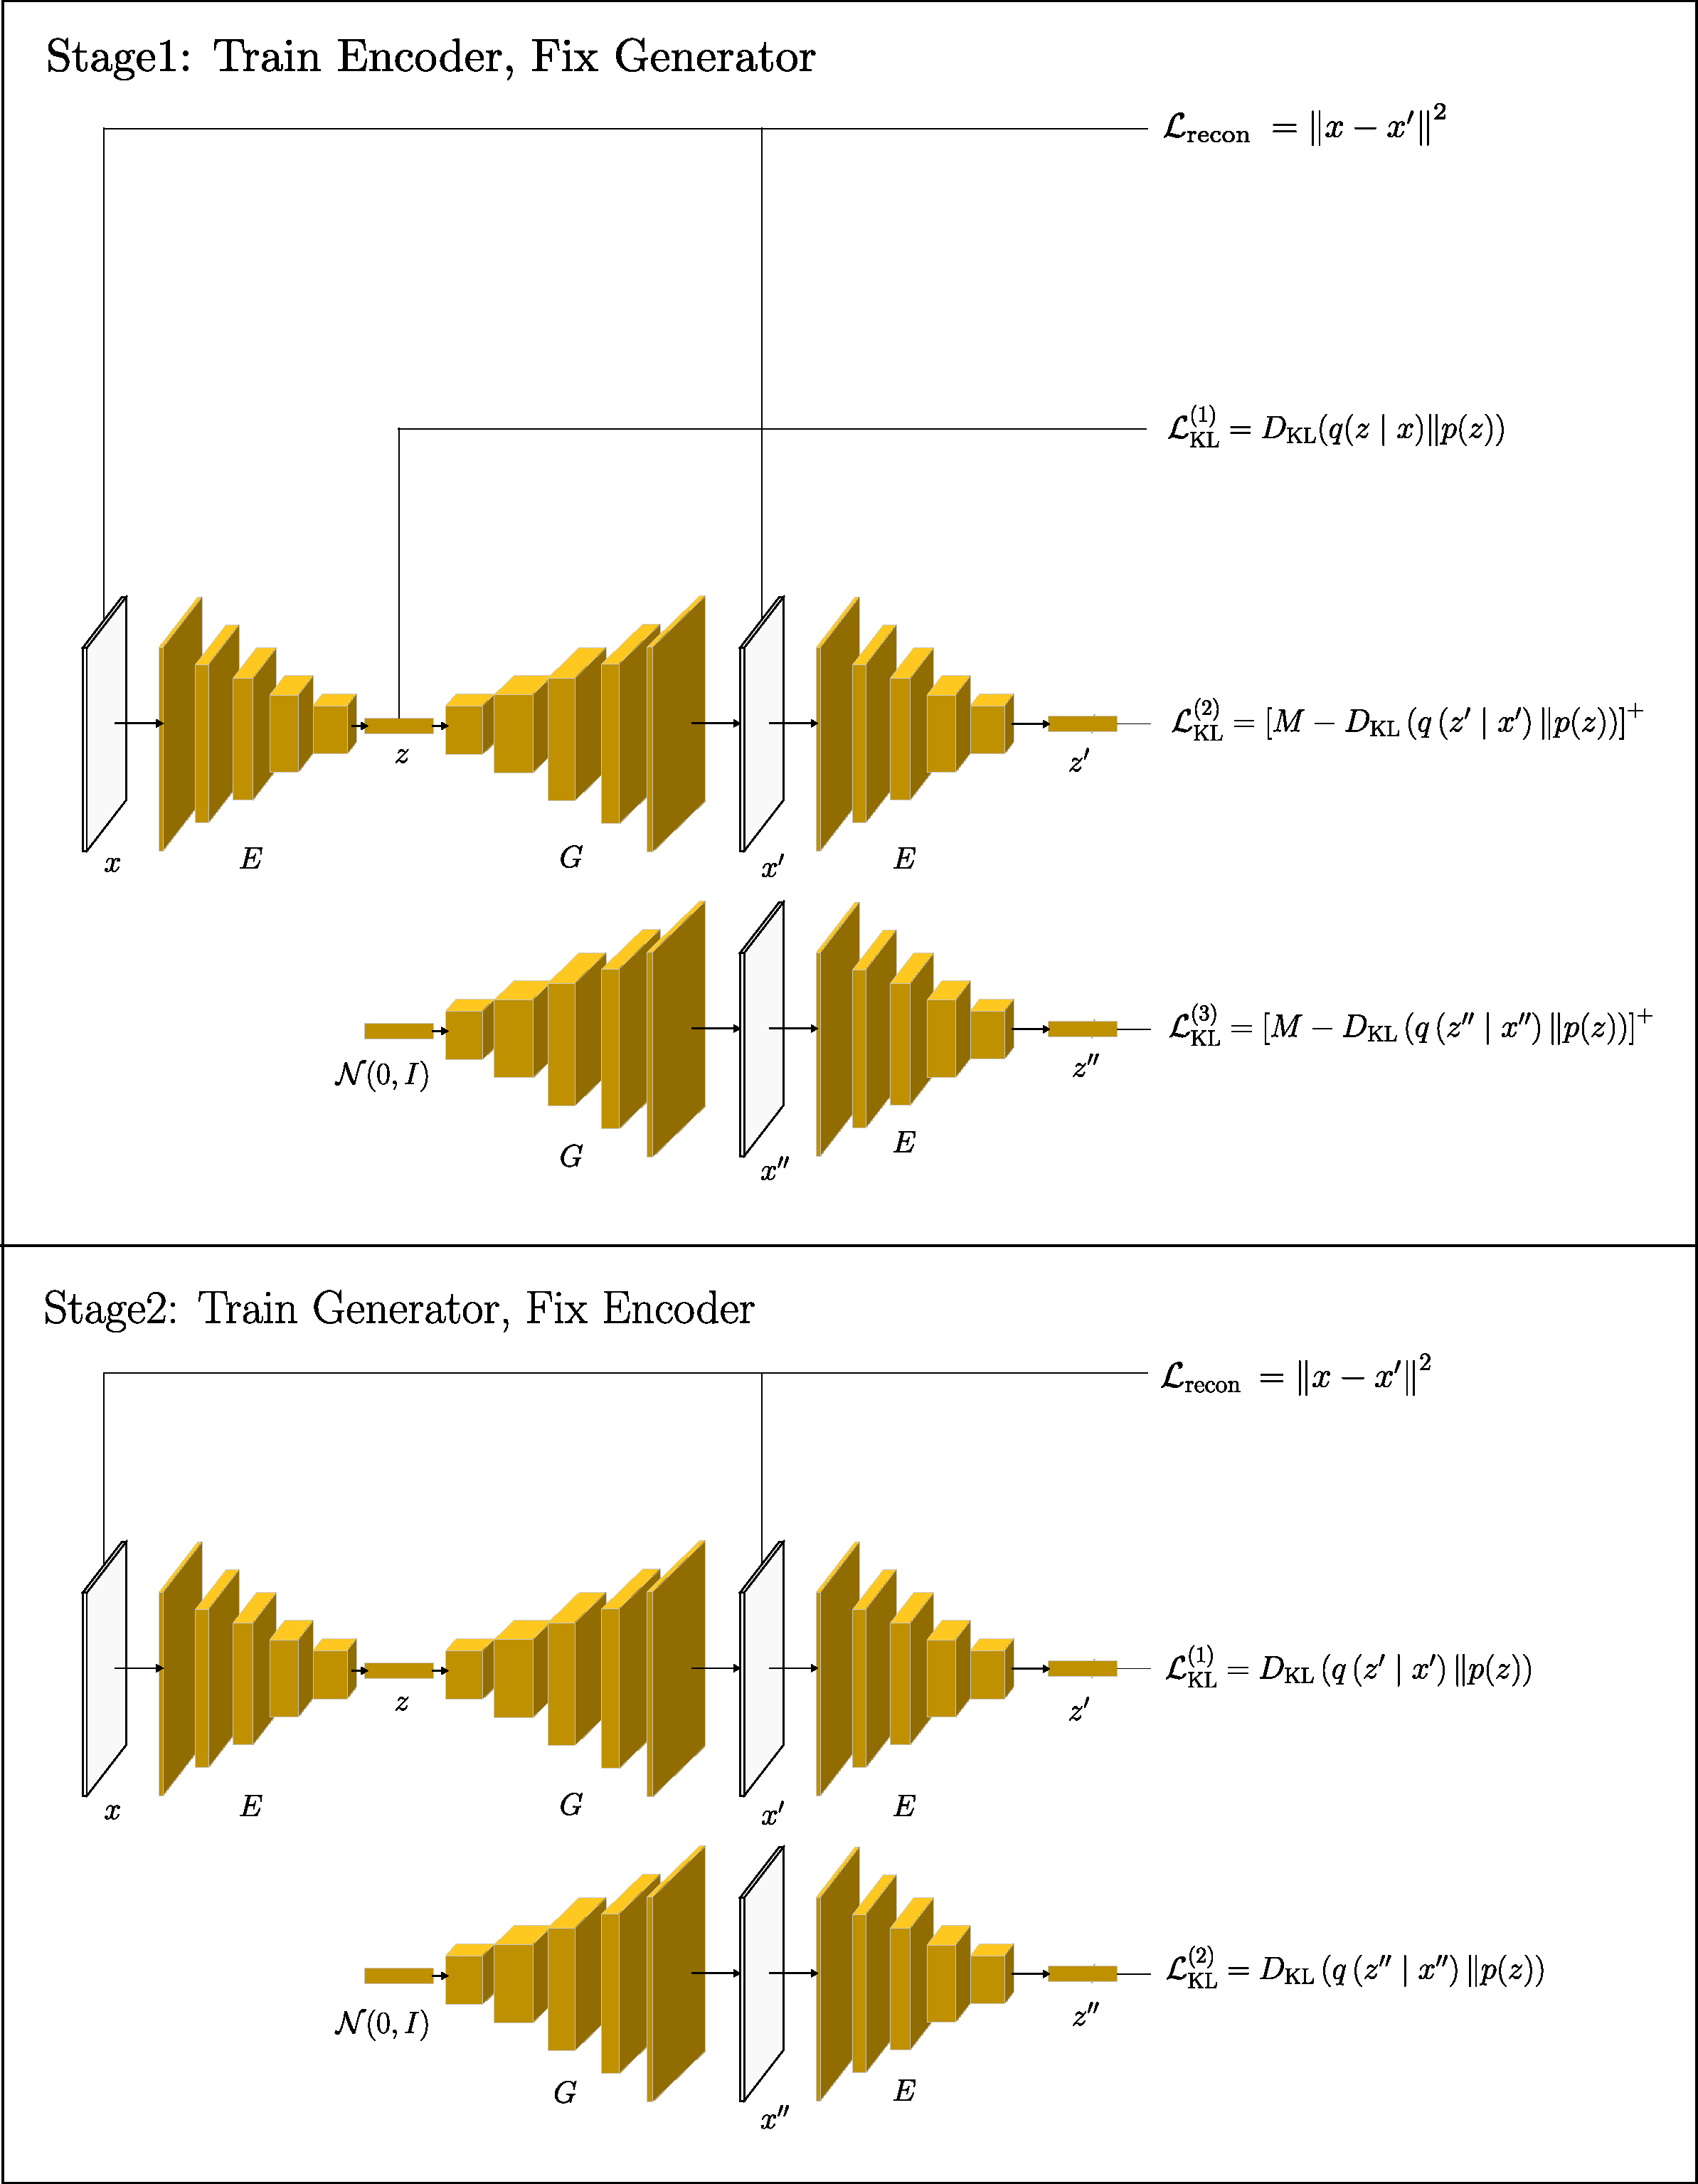
\includegraphics[width=\textwidth]{./assets/lraad_model.pdf}
    \caption{The Training Pipeline of LRAAD}
    \label{fig:lraad}
\end{figure}

\subsection{模型训练}
首先，LRAAD的流程以编码器开始。编码器接收一张频谱图（通常是梅尔频谱图）作为输入，并将其转换为潜在空间的表示。这个表示是对输入频谱图的抽象表达，记为 z。编码器的目标是通过学习将正常数据的潜在表示尽可能接近标准正态分布，而将异常数据的潜在表示远离标准正态分布。这样的训练过程可以使得编码器能够更好地区分正常和异常数据。

接下来是生成器的阶段。生成器接收编码器生成的潜在变量 z，并将其映射回频谱图的梅尔频谱域，生成尽可能真实的频谱图。生成器的目标是通过学习将潜在变量映射到与正常数据频谱图相似的图像，从而提供优质的正常数据样本来优化编码器的学习过程。生成器的训练与编码器交替进行，利用对抗学习的框架来不断提高生成器的生成能力。

下面详细介绍LRAAD模型的训练过程及其损失函数设计。

\subsubsection{编码器训练}

编码器的训练目标是将正常数据的潜在表示$z$尽可能接近标准正态分布，同时将生成数据的潜在表示$z^\prime$和$z^{\prime\prime}$远离标准正态分布。为了实现这一目标，编码器需要学习如何在潜在空间中对输入频谱图进行有效的表示。通过对抗学习的方式，编码器不断优化其输出，使得正常数据和异常数据在潜在空间中实现分离。编码器的训练损失主要包括KL散度损失和重构损失两部分。

\textbf{KL散度损失：} KL散度损失用于衡量编码器生成的潜在表示 z 与标准正态分布的差异。在LRAAD模型中，KL散度损失通过计算潜在表示的分布与标准正态分布$p(z)=\mathcal{N}(0, I)$之间的KL散度来评估它们的相似性。对于正常数据，编码器的目标是最小化其KL散度损失，使其潜在表示与标准正态分布尽可能接近。对于生成数据，编码器的目标是最大化其KL散度损失，使其潜在表示远离标准正态分布。这样的训练方式可以促使编码器将正常数据和异常数据在潜在空间中分离开来，从而使得编码器可以充当判别器的角色，有效区分正常数据和异常数据。

\begin{equation}
  \mathcal{L}_{\mathrm{KL}}=D_{\mathrm{KL}}(q(z \mid x) \| p(z)) + [M - D_{\mathrm{KL}}\left(q\left(z^{\prime} \mid x^{\prime}\right) \| p(z)\right)]^{+} + [M - D_{\mathrm{KL}}\left(q\left(z^{\prime \prime} \mid x^{\prime \prime}\right) \| p(z)\right)]^{+}
\end{equation}

其中，$q(z \mid x)$表示编码器编码正常数据$x$的潜在表示的分布，$q(z^\prime \mid x^\prime)$和$q(z^{\prime\prime} \mid x^{\prime\prime})$分别表示编码器编码生成数据$x^\prime$和$x^{\prime\prime}$的潜在表示的分布。$p(z)$表示标准正态分布，记为$\mathcal{N}(0, I)$。$D_{\mathrm{KL}}$表示KL散度，$[M - D_{\mathrm{KL}}]^{+}$表示KL散度的修正项，其中$M$是一个超参数，用于控制KL散度的上限。

\textbf{重构损失：}重构损失衡量的是输入数据与重建数据之间的差异。在LRAAD模型中，重构损失用于确保编码器生成的潜在表示 z 能够准确地重建原始输入频谱图 x。具体来说，编码器生成潜在表示$z$后，通过生成器将$z$反向映射回频谱图域，生成重建的频谱图$x^\prime$。重构损失的目标是最小化$x$与$x^\prime$之间的差异，常用的重构损失函数是均方误差（Mean Squared Error，MSE）, 其计算公式如下：

\begin{equation}
\mathcal{L}_{\text {recon }}=\left\|x-x^{\prime}\right\|^2
\end{equation}

总的损失函数为：

\begin{equation} \label{eq:encoder_loss}
  \mathcal{L_E}=\beta_{\text {KL }} \cdot\mathcal{L}_{\text {KL }}+\beta_{\text {recon }} \cdot\mathcal{L}_{\text {recon }}
\end{equation}

\subsubsection{生成器训练}
生成器的目标与判别器相反，即让判别器将自己生成的样本判别为真实样本。生成器的训练过程始于接收编码器编码正常数据$x$生成的潜在变量$z$和在正态分布中采样的潜在变量$z_{p}$。生成器将潜在变量$z$和$z_{p}$作为输入，并通过一系列神经网络层，逐步将其反向映射到频谱图的梅尔频谱域，生成频谱图$x^\prime$和$x^{\prime \prime}$。生成器的目标是生成的频谱图$x^\prime$和$x^{\prime \prime}$能够尽可能真实地接近正常数据的频谱图。在训练过程中，生成器和编码器通过对抗学习的框架相互优化，使得生成器不断提高生成频谱图的质量，同时优化编码器的判别能力。生成器的训练损失主要包括对抗性损失和重构损失两部分。

\textbf{对抗性损失：}对抗性损失用于衡量生成器生成的频谱图$x^\prime$和$x^{\prime \prime}$与正常数据频谱图之间的差异。在LRAAD模型中，对抗性损失通过判别器$D$来评估生成器生成的频谱图的真实性。判别器的目标是区分正常数据频谱图和生成的频谱图，使得生成器生成的频谱图更加真实。对抗性损失的计算公式如下：

\begin{equation}
  \mathcal{L}_{\text {adv }}=D_\mathrm{KL}(q(z^\prime \mid x^\prime) \| p(z)) + D_\mathrm{KL}(q(z^{\prime\prime} \mid x^{\prime\prime}) \| p(z))
\end{equation}

\textbf{重构损失：}重构损失用于衡量生成的频谱图 x' 与真实输入频谱图 x 之间的差异。这一损失确保生成器能够准确地还原输入频谱图的特征。重构损失通常采用均方误差（MSE）来计算：

\begin{equation} \label{eq:generator_loss}
  \mathcal{L}_{\text {recon }}=\left\|x-x^{\prime}\right\|^2
\end{equation}

总的损失函数为：

\begin{equation}
  \mathcal{L_G}=\beta_{\text {adv }} \cdot\mathcal{L}_{\text {adv }}+\beta_{\text {recon }} \cdot\mathcal{L}_{\text {recon }}
\end{equation}

LRAAD模型的训练过程如表\ref{tab:training}所示。在训练过程中，编码器和生成器通过对抗学习的方式相互优化，使得编码器能够学习到正常数据的潜在表示，并将其映射到标准正态分布，同时将异常数据的潜在表示映射到偏离标准正态分布的区域。生成器的目标是生成尽可能真实的频谱图，使得编码器能够更好地区分正常数据和异常数据。通过这种方式，LRAAD模型能够有效地拟合正常数据的分布。

\begin{table}[H]
    \centering
    \begin{tabular}{l}
        \toprule
        \label{tab:training}
        {\textbf{Algorithm} Training LRAAD model} \\
        \midrule
        1: Initialize network parameters \\
        2: \quad {\textbf{For} number of epochs \textbf{do}} \\
        3: \quad\quad Random mini-batch $X$ from dataset \\
        4: \quad\quad Compute latent representation of $X$: $Z = E(X)$ \\
        5: \quad\quad Sample $Z_p$ from prior distribution $p(z)=\mathcal{N}(0, I)$ \\
        6: \quad\quad Compute reconstructed spectrogram of $Z$ and $Z_p$: $X^\prime = G(Z)$, $X^{\prime\prime} = G(Z_p)$ \\
        7: \quad\quad Compute latent representation of $X^\prime$ and $X^{\prime\prime}$: $Z^\prime = E(X^\prime)$, $Z^{\prime\prime} = E(X^{\prime\prime})$ \\
        8: \quad\quad Compute Encoder loss $\mathcal{L}_E$ according to Eq. \ref{eq:encoder_loss} \\
        9: \quad\quad Update Encoder parameters by minimizing $\mathcal{L}_E$ \\
        10: \quad\quad Compute Generator loss $\mathcal{L}_G$ according to Eq. \ref{eq:generator_loss} \\
        11: \quad\quad Update Generator parameters by minimizing $\mathcal{L}_G$ \\
        12: \quad {\textbf{End For}} \\


        \bottomrule
    \end{tabular}
\end{table}


\subsection{异常检测}

在训练完成后，我们可以使用训练好的生成器和编码器来计算每个输入频谱图的异常分数。异常分数用于衡量输入频谱图与正常数据分布之间的差异，从而识别出潜在的异常。

我们使用重构误差作为异常分数来衡量输入数据与模型生成数据之间的差异，从而识别潜在的异常。具体地，对于给定的梅尔频谱图输入$x$，我们首先通过编码器将其映射到潜在空间中得到潜在变量$z$。然后，使用生成器从潜在变量$z$生成重构的频谱图$x^\prime$。重构的频谱图$x^\prime$与原始输入$x$的L1误差作为异常分数。其计算公式如下：

\begin{equation}
\mathcal{A}(x)=\left\|x-G\left(E(x)\right)\right\|_1
\end{equation}
其中，$\mathcal{A}(x)$是输入梅尔频谱图$x$的异常分数，$E(x)$是编码器$E$的输出的潜在变量，$G(E(x))$是生成器$G$从潜在变量生成的重构频谱图。重构误差越大，表示重构的频谱图与原始输入之间的差异越大，可能表明输入的频谱图具有异常或不正常的特征。

在实际应用中，我们可以设置一个阈值来判断重构误差是否超过正常范围，并将超过阈值的样本标记为异常。通过这种方式，我们可以使用重构误差作为异常分数来进行声学异常检测，从而识别出潜在的异常或不正常的电力设备声学信号。

% \section{实验：Experiments}
\section{Experiments}
本节我们将介绍实验的设置和结果。我们首先介绍实验的数据集和预处理方法，然后详细描述实验的设置和评估指标，最后给出实验结果和分析。

\subsection{Dataset}
本实验采用的数据集是从中国某\(\pm\)800kV特高压换流站的换流阀实测声音数据。这些数据是通过在换流站安装的传声器实时采集得到的，用于监测换流阀在运行过程中产生的声音信号。这些数据包含了换流站在正常运行状态下以及可能存在异常情况下记录的声音信号。在正常运行状态下，换流站产生的声音信号应当是稳定的，并且不会出现异常噪音。而在异常情况下，可能会出现各种故障或异常情况，例如设备摩擦、松动、电弧放电等，这些异常情况可能会导致声音信号的突变或异常增加。因此，通过分析和识别声音信号中的异常模式，可以帮助监测和诊断换流站设备的健康状况。

该数据集包含了一系列声音信号的录音文件，录音文件以 WAV 格式存储，每个文件记录了在不同时间点下换流站产生的声音信号。每个录音文件的采样频率为44.1Hz，持续时间为10秒。在数据集的收集过程中，我们尽可能涵盖了换流站设备可能遇到的各种正常和异常情况，以确保数据集的多样性和代表性。同时，我们还对录音文件进行了标注，将正常状态和异常状态的声音信号区分开来，以便于实验和分析。


换流阀的视在功率范围为400MVA到1000MVA，根据视在功率的不同，将实测声音数据分为六个子集，分别记为Dataset1至Dataset6。每个数据集对应一个特定的视在功率范围，具体如下：

\begin{table}[h!]
\centering
\begin{tabular}{c c}
\toprule
\textbf{数据集} & \textbf{视在功率范围 (MVA)} \\
\midrule
Dataset1 & 400 - 500 \\
Dataset2 & 500 - 600 \\
Dataset3 & 600 - 700 \\
Dataset4 & 700 - 800 \\
Dataset5 & 800 - 900 \\
Dataset6 & 900 - 1000 \\
\bottomrule
\end{tabular}
\caption{视在功率范围对应的数据集}
\label{table:datasets}
\end{table}


为了进行实验，我们将每个录音文件切分为多个长度为1.36秒的音频片段，然后将每个音频片段转换为对应的梅尔频谱图。梅尔频谱图是声音信号的一种常用表示形式，它可以更好地反映声音信号的频谱特征。我们使用梅尔频谱图作为模型的输入，以便于模型学习和分析声音信号的频谱特征。对于每个梅尔频谱图，我们对其进行对数变换和归一化处理，以便于模型训练和优化。

\subsection{Data Preprocessing}

在进行声学信号的异常检测实验时，数据预处理是非常关键的一步，它直接影响到后续模型的训练和异常检测的准确性。下面是我们对实验数据进行的详细预处理步骤：


为了更好地处理数据和提取特征，我们首先将长时间的音频信号分段为较短的片段。这可以通过滑动窗口的方式进行，每个窗口包含一段时间内的音频数据。这样做的目的是使得数据更易于处理，并且可以更精确地捕获声音的时间特征。


对于每个音频分段，我们使用梅尔频率倒谱系数（Mel Frequency Cepstral Coefficients，MFCC）来表示其频谱特征。梅尔频谱是在横坐标上使用Mel刻度，纵坐标上是功率谱的一种表示方式，更符合人类听觉感知的特性。我们使用Librosa等库来进行梅尔频谱转换，将每个音频分段转换为对应的梅尔频谱图。 对于得到的梅尔频谱图，我们对其进行对数变换。这一步骤可以有效地增强低频特征的信息，减少高频特征的干扰，使得数据更加平滑和稳定。

接下来，我们对经过对数变换的梅尔频谱图进行归一化处理。归一化的目的是将数据缩放到一个统一的范围内，以避免不同特征之间的数值差异对模型训练造成影响。我们使用最小-最大归一化来处理数据。

\subsection{Experimental Settings}

LRAL-AD 模型包含编码器、生成器和判别器三个主要部分。编码器使用了由 CAE 提出的架构，包括五个卷积层，负责将输入的梅尔频谱图映射到潜在空间中的均值和方差。生成器则采用了 DCGAN 提出的架构，包括五个反卷积层，用于将潜在变量映射回梅尔频谱域，实现频谱图的重建。判别器也采用了 DCGAN 的架构，包括五个卷积层，用于判断输入的频谱图是真实数据还是生成数据。这种架构的设计旨在平衡编码器的特征提取能力、生成器的重建能力和判别器的区分能力，从而提高异常检测的准确性和鲁棒性。

在训练 LRAAD 模型时，我们需要设置多个超参数来调节模型的性能。例如，编码器和生成器的学习率、损失函数的权重系数（如重构损失、对抗损失、KL 散度损失的权重）、潜在空间的维度大小、训练的迭代次数等。这些超参数的选择对模型的训练和性能具有重要影响，需要通过实验和验证来确定最佳的超参数组合。在实验中，我们采用的超参数设置如Table \ref{tab:params}所示：


\begin{table}[htbp]
    \centering
    \caption{LRAAD Model Hyperparameter Settings}
    \label{tab:params}
    \begin{tabular}{lr}
        \toprule
        \textbf{Hyperparameter} & \textbf{Setting} \\
        \midrule
        Latent Space Dimension & 32 \\
        Learning Rate (Encoder) & 0.0002 \\
        Learning Rate (Generator) & 0.0002 \\
        Loss Weight (Reconstruction) & 1 \\
        Loss Weight (Adversarial) & 1 \\
        Loss Weight (KL Divergence) & 1 \\
        M (KL Divergence Limit) & 100 \\
        Training Epochs & 100 \\
        Batch Size & 32 \\
        Dataset Split & 80\% Training, 30\% Testing \\
        \bottomrule
    \end{tabular}
\end{table}


% \subsection{评估指标：Evaluation Metrics}
\subsection{Evaluation Metrics}
在实验中，评估指标是对模型性能进行客观量化和比较的重要标准。我们主要使用了AUC（Area Under the ROC Curve）指标来评估异常检测模型的效果。

ROC曲线（Receiver Operating Characteristic Curve）：ROC曲线是用于评估二分类模型性能的图形工具，横轴表示假阳性率（False Positive Rate，FPR），纵轴表示真阳性率（True Positive Rate，TPR）。ROC曲线能够直观展示在不同阈值下模型的真阳性率与假阳性率之间的权衡关系。一般来说，ROC曲线越接近左上角（TPR高、FPR低），说明模型性能越好，对异常检测问题来说，ROC曲线的面积（AUC）越大，表示模型对于正常和异常样本的区分能力越强。

AUC（Area Under Curve）：AUC是ROC曲线下方的面积，用于衡量模型分类效果的一个总体指标。AUC的取值范围在0.5到1之间，其中0.5表示模型性能等同于随机分类，1表示完美分类。在异常检测任务中，AUC值越接近1，说明模型对正常和异常样本的区分能力越强，具有更好的检测准确度。

ROC 曲线和 AUC 指标是评估异常检测模型性能的重要指标，能够直观地反映模型在识别异常样本和正常样本方面的表现，并帮助比较不同模型的性能优劣。

% \subsection{实验结果：Experimental Results}
\subsection{Experimental Results}
为验证LRAAD模型在异常检测领域的检测性能，本实验将LRAAD模型与CAE、AnoGAN、GANomaly等经典异常检测模型进行了对比实验。实验结果表明，LRAAD模型在异常检测任务上取得了更好的性能表现，具有更高的AUC和p-AUC值，能够更准确地识别出异常样本。

Figure \ref{fig:roc_curve}展示了LRAAD模型与其他模型在异常检测任务上的ROC曲线比较。从图中可以看出，LRAAD模型的ROC曲线处于其他模型的上方，AUC值更高，表明LRAAD模型具有更好的性能表现。表\ref{tab:auc}、表\ref{tab:p-auc-03}、表\ref{tab:p-auc-02}和表\ref{tab:p-auc-01}分别展示了不同模型在不同数据集上的AUC和p-AUC值的比较。从表中可以看出，LRAAD模型在所有数据集上均取得了更高的AUC和p-AUC值，相比其他模型具有更好的异常检测性能。

\begin{table}[H]
    \centering
    \begin{tabular}{cccccc}
        \toprule
        Dataset & CAE & VAE & f-AnoGAN & GANomaly & LRAAD(Our) \\
        \midrule
        Dataset1 & 0.8975 & 0.8662 & 0.8400 & 0.8966 & \textbf{0.9361} \\
        Dataset2 & 0.8911 & 0.8652 & 0.8560 & 0.9195 & \textbf{0.9475} \\
        Dataset3 & 0.9266 & 0.8958 & 0.8662 & 0.9266 & \textbf{0.9607} \\
        Dataset4 & 0.9087 & 0.8868 & 0.8654 & 0.9333 & \textbf{0.9626} \\
        Dataset5 & 0.8962 & 0.8965 & 0.8910 & 0.9511 & \textbf{0.9721} \\
        Dataset6 & 0.8523 & 0.8178 & 0.8126 & 0.8270 & \textbf{0.8674} \\
        \bottomrule
    \end{tabular}
    \caption{AUC Comparison of Different Models on Different Datasets}
    \label{tab:auc}
\end{table}


\begin{table}[H]
    \centering
    \begin{tabular}{cccccc}
        \toprule
        Dataset & CAE & VAE & f-AnoGAN & GANomaly & LRAAD(Our) \\
        \midrule
        Dataset1 & 0.6664 & 0.5824 & 0.5161 & 0.7232 & \textbf{0.7930} \\
        Dataset2 & 0.6394 & 0.5559 & 0.5487 & 0.7843 & \textbf{0.8430} \\
        Dataset3 & 0.7605 & 0.6576 & 0.5935 & 0.8076 & \textbf{0.8639} \\
        Dataset4 & 0.6972 & 0.6252 & 0.5790 & 0.8164 & \textbf{0.8342} \\
        Dataset5 & 0.6529 & 0.6569 & 0.6423 & 0.8705 & \textbf{0.8866} \\
        Dataset6 & 0.5262 & 0.4656 & 0.4589 & 0.5243 & \textbf{0.6335} \\
        \bottomrule
    \end{tabular}
    \caption{p-AUC Comparison of Different Models on Different Datasets (FPR<0.3)}
    \label{tab:p-auc-03}
\end{table}

\begin{table}[H]
    \centering
    \begin{tabular}{cccccc}
        \toprule
        Dataset & CAE & VAE & f-AnoGAN & GANomaly & LRAAD(Our) \\
        \midrule
        Dataset1 & 0.5431 & 0.4503 & 0.3809 & 0.6417 & \textbf{0.7078} \\
        Dataset2 & 0.5355 & 0.4192 & 0.4037 & 0.7324 & \textbf{0.7865} \\
        Dataset3 & 0.7041 & 0.5225 & 0.4598 & 0.7496 & \textbf{0.8176} \\
        Dataset4 & 0.6142 & 0.5014 & 0.4532 & 0.7609 & \textbf{0.8173} \\
        Dataset5 & 0.5465 & 0.5390 & 0.5371 & \textbf{0.8332} & 0.8115 \\
        Dataset6 & 0.3801 & 0.3190 & 0.3227 & 0.3935 & \textbf{0.5377} \\

        \bottomrule
    \end{tabular}
    \caption{p-AUC Comparison of Different Models on Different Datasets (FPR<0.2)}
    \label{tab:p-auc-02}
\end{table}

\begin{table}[H]
    \centering
    \begin{tabular}{cccccc}
        \toprule
        Dataset & CAE & VAE & f-AnoGAN & GANomaly & LRAAD(Our) \\
        \midrule
        Dataset1 & 0.3640 & 0.2736 & 0.2261 & 0.5268 & \textbf{0.5629} \\
        Dataset2 & 0.4405 & 0.2472 & 0.2318 & 0.6353 & \textbf{0.6658} \\
        Dataset3 & 0.6024 & 0.3372 & 0.2651 & 0.6810 & \textbf{0.7020} \\
        Dataset4 & 0.5487 & 0.3345 & 0.3136 & 0.6635 & \textbf{0.6993} \\
        Dataset5 & 0.4090 & 0.3700 & 0.3964 & \textbf{0.7626} & 0.7400 \\
        Dataset6 & 0.2168 & 0.1566 & 0.1624 & 0.2330 & \textbf{0.3791}\\

        \bottomrule
    \end{tabular}
    \caption{p-AUC Comparison of Different Models on Different Datasets (FPR<0.1)}
    \label{tab:p-auc-01}
\end{table}

\begin{figure}
  \centering
  \includegraphics[width=0.45\linewidth]{./experiments/ssva1/roc_curve.pdf}
  \hfill
  \includegraphics[width=0.45\linewidth]{./experiments/ssva2/roc_curve.pdf}
  \hfill
  \includegraphics[width=0.45\linewidth]{./experiments/ssva3/roc_curve.pdf}
  \hfill
  \includegraphics[width=0.45\linewidth]{./experiments/ssva4/roc_curve.pdf}
  \hfill
  \includegraphics[width=0.45\linewidth]{./experiments/ssva5/roc_curve.pdf}
  \hfill
  \includegraphics[width=0.45\linewidth]{./experiments/ssva6/roc_curve.pdf}
  \caption{ROC Curves of Different Models on Different Datasets}
\end{figure}

\section{Conclusion}
 LRAAD模型通过引入编码器和生成器两个模块，实现了在潜在空间中的对抗学习，并使用编码器作为判别器，使正常数据的潜在表示与标准正态分布的KL散度最小化，而生成数据的潜在表示与标准正态分布的KL散度最大化，从而实现了编码器对正常数据和异常数据在潜在空间中的有效分离。

 LRAAD模型在AUC指标和p-AUC指标上都实现了较高的性能，这表明模型具有较好的异常声音检测能力，可以有效地区分正常声音和异常声音，有助于及时发现换流阀的潜在问题和故障。通过与其他经典模型如CAE、VAE、f-AnoGAN和GANomaly的对比实验，LRAAD模型在异常检测领域的表现明显优于其他模型，这验证了模型的有效性和实用性。LRAAD模型通过引入潜在变量正则化对抗学习，提高了模型对异常声音的敏感性和识别能力，从而更好地适应实际工业生产中的异常检测任务。

 但是，仍有一些需要改进和深入探讨的地方,具体如下:第一，可以探索更多的损失函数组合和优化策略，以提高模型的鲁棒性和泛化能力。第二,论文没有对模型各部分超参数的敏感性进行分析。对模型各部分超参数的敏感性分析,有助于把握模型行为，能让我们更好地理解不同超参数对模型表现的影响,从而指导参数调优,获得最佳性能。第三,异常分数计算的方式较为简单,或许可以探索更复杂的异常分数度量方式。当前的异常分数仅利用了重建误差,将来可以考虑引入其他先验知识,设计更合理的异常分数函数。第四,可以进一步分析LRAAD在不同类型异常声音上的表现,看看是否存在一些模式偏好。对于复杂的工业场景,不同类型的异常可能需要专门的建模方式,了解当前模型的偏好有助于指导下一步改进方向。第四,模型的可解释性有待加强,这对异常检测任务很重要。高可解释性能让异常结果更易被人类理解和判断,从而提高异常检测系统的可信赖性。

\bibliography{references}

\end{document}

